\documentclass[11pt,a4paper]{article}

\usepackage[T1]{fontenc}
\usepackage[utf8]{inputenc}
\usepackage[english]{babel}
\usepackage[sc]{mathpazo}
\linespread{1.05}
\usepackage{microtype}
\usepackage[a4paper,margin=2.5cm]{geometry}
\usepackage{amsmath,amssymb,mathtools}
\usepackage{graphicx}
\usepackage{booktabs,tabularx,array}
\usepackage{enumitem}
\usepackage[font=small,labelfont=bf,labelsep=colon]{caption}
\usepackage{xcolor}
\definecolor{blueI}{HTML}{2A78D6}
\definecolor{orangeJ}{HTML}{EB6834}
\definecolor{ink}{HTML}{0B0B0B}
\definecolor{ink2}{HTML}{52514E}
\usepackage[hidelinks]{hyperref}
\usepackage{xr-hyper}
\externaldocument[crest-]{../crests/crest_geometry}[../crests/crest_geometry.pdf]
% Floats go where they fit, so that few pages hold a float alone.
\makeatletter
\def\fps@figure{htbp}
\def\fps@table{htbp}
\makeatother
\renewcommand{\topfraction}{0.85}
\renewcommand{\bottomfraction}{0.6}
\renewcommand{\textfraction}{0.1}
\renewcommand{\floatpagefraction}{0.75}
\setcounter{topnumber}{3}
\setcounter{bottomnumber}{2}
\setcounter{totalnumber}{4}

\newcommand{\Hgeo}{H_{\mathrm{geo}}}
\newcommand{\code}[1]{\texttt{#1}}

% Numbers of the flight part (report.py --part model): a frozen copy.
% Generated by report.py: do not edit.
\providecommand{\Hmod}{H_{\mathrm{mod}}}
\providecommand{\Hdyn}{H_{\mathrm{dyn}}}
\providecommand{\Hroute}{H_{\mathrm{route}}}
\newcommand{\flAlphaEnd}{0.98}
\newcommand{\flFloorM}{100}
\newcommand{\flNBoot}{1000}
\newcommand{\flNReal}{3}
\newcommand{\flMinFlights}{30}
\newcommand{\flMinRows}{100}
\newcommand{\flCandPara}{67\,646}
\newcommand{\flStatOkPara}{25\,460}
\newcommand{\flStatDtPara}{3\,207}
\newcommand{\flStatOpeningPara}{10\,505}
\newcommand{\flStatRegionPara}{28\,404}
\newcommand{\flSelAlpsPara}{23\,320}
\newcommand{\flSelPyrPara}{2\,140}
\newcommand{\flCandHang}{2\,194}
\newcommand{\flStatOkHang}{795}
\newcommand{\flStatDtHang}{393}
\newcommand{\flStatOpeningHang}{627}
\newcommand{\flStatRegionHang}{377}
\newcommand{\flSelAlpsHang}{784}
\newcommand{\flSelPyrHang}{11}
\newcommand{\flNOneHzAlpsPara}{15884}
\newcommand{\flNPhaseFlightsAlpsPara}{15189}
\newcommand{\flVGlideAlpsPara}{10.2}
\newcommand{\flVGlideAlpsParaLo}{10.2}
\newcommand{\flVGlideAlpsParaHi}{10.2}
\newcommand{\flVGlideKmhAlpsPara}{37}
\newcommand{\flVGlideKmhAlpsParaLo}{37}
\newcommand{\flVGlideKmhAlpsParaHi}{37}
\newcommand{\flGlideNAlpsPara}{334\,886}
\newcommand{\flGlideMeanAlpsPara}{281}
\newcommand{\flGlideLawAlpsPara}{Lomax}
\newcommand{\flGlideParamAAlpsPara}{10.11}
\newcommand{\flGlideParamAAlpsParaLo}{9.69}
\newcommand{\flGlideParamAAlpsParaHi}{10.57}
\newcommand{\flGlideParamBAlpsPara}{2555}
\newcommand{\flGlideParamBAlpsParaLo}{2437}
\newcommand{\flGlideParamBAlpsParaHi}{2685}
\newcommand{\flGlideMeanFitAlpsPara}{281}
\newcommand{\flGlideMeanFitAlpsParaLo}{280}
\newcommand{\flGlideMeanFitAlpsParaHi}{283}
\newcommand{\flGlideThetaAlpsPara}{280}
\newcommand{\flGlideAicLomaxAlpsPara}{0}
\newcommand{\flGlideAicExpAlpsPara}{3417}
\newcommand{\flGlideAicWeibullAlpsPara}{1776}
\newcommand{\flGlideAicGammaAlpsPara}{2635}
\newcommand{\flPauseNAlpsPara}{323\,423}
\newcommand{\flPauseMeanAlpsPara}{158}
\newcommand{\flPauseLawAlpsPara}{Weibull}
\newcommand{\flPauseParamAAlpsPara}{1.150}
\newcommand{\flPauseParamAAlpsParaLo}{1.145}
\newcommand{\flPauseParamAAlpsParaHi}{1.154}
\newcommand{\flPauseParamBAlpsPara}{165}
\newcommand{\flPauseParamBAlpsParaLo}{165}
\newcommand{\flPauseParamBAlpsParaHi}{166}
\newcommand{\flPauseMeanFitAlpsPara}{158}
\newcommand{\flPauseMeanFitAlpsParaLo}{157}
\newcommand{\flPauseMeanFitAlpsParaHi}{158}
\newcommand{\flPauseThetaAlpsPara}{157}
\newcommand{\flPauseAicLomaxAlpsPara}{9134}
\newcommand{\flPauseAicExpAlpsPara}{9105}
\newcommand{\flPauseAicWeibullAlpsPara}{0}
\newcommand{\flPauseAicGammaAlpsPara}{1796}
\newcommand{\flNAlpsPara}{23320}
\newcommand{\flNPathsAlpsPara}{12981}
\newcommand{\flTauMaxAlpsPara}{2182}
\newcommand{\flTauFloorAlpsPara}{10}
\newcommand{\flHGeoAlpsPara}{0.934}
\newcommand{\flHGeoAlpsParaLo}{0.930}
\newcommand{\flHGeoAlpsParaHi}{0.940}
\newcommand{\flStartGeoAlpsPara}{11}
\newcommand{\flStartGeoAlpsParaLo}{11}
\newcommand{\flStartGeoAlpsParaHi}{13}
\newcommand{\flHModAlpsPara}{0.892}
\newcommand{\flHModAlpsParaLo}{0.888}
\newcommand{\flHModAlpsParaHi}{0.896}
\newcommand{\flStartModAlpsPara}{10}
\newcommand{\flStartModAlpsParaLo}{10}
\newcommand{\flStartModAlpsParaHi}{10}
\newcommand{\flHDynAlpsPara}{0.901}
\newcommand{\flHDynAlpsParaLo}{0.901}
\newcommand{\flHDynAlpsParaHi}{0.902}
\newcommand{\flStartDynAlpsPara}{10}
\newcommand{\flStartDynAlpsParaLo}{10}
\newcommand{\flStartDynAlpsParaHi}{10}
\newcommand{\flHRouteAlpsPara}{0.929}
\newcommand{\flHRouteAlpsParaLo}{0.929}
\newcommand{\flHRouteAlpsParaHi}{0.930}
\newcommand{\flStartRouteAlpsPara}{10}
\newcommand{\flStartRouteAlpsParaLo}{10}
\newcommand{\flStartRouteAlpsParaHi}{10}
\newcommand{\flHTenAlpsPara}{0.926}
\newcommand{\flHTenAlpsParaLo}{0.924}
\newcommand{\flHTenAlpsParaHi}{0.928}
\newcommand{\flHTenLastAlpsPara}{8537}
\newcommand{\flHStraightAlpsPara}{0.945}
\newcommand{\flHStraightAlpsParaLo}{0.941}
\newcommand{\flHStraightAlpsParaHi}{0.947}
\newcommand{\flNullDHStraightAlpsPara}{0.044}
\newcommand{\flNullDHStraightAlpsParaLo}{0.040}
\newcommand{\flNullDHStraightAlpsParaHi}{0.046}
\newcommand{\flNullGapStraightAlpsPara}{44}
\newcommand{\flNullGapStraightAlpsParaLo}{40}
\newcommand{\flNullGapStraightAlpsParaHi}{47}
\newcommand{\flHRandomAlpsPara}{0.849}
\newcommand{\flHRandomAlpsParaLo}{0.844}
\newcommand{\flHRandomAlpsParaHi}{0.852}
\newcommand{\flNullDHRandomAlpsPara}{$-$0.052}
\newcommand{\flNullDHRandomAlpsParaLo}{$-$0.057}
\newcommand{\flNullDHRandomAlpsParaHi}{$-$0.049}
\newcommand{\flNullGapRandomAlpsPara}{$-$53}
\newcommand{\flNullGapRandomAlpsParaLo}{$-$57}
\newcommand{\flNullGapRandomAlpsParaHi}{$-$50}
\newcommand{\flHModOldAlpsPara}{0.882}
\newcommand{\flHModOldAlpsParaLo}{0.877}
\newcommand{\flHModOldAlpsParaHi}{0.885}
\newcommand{\flPctInterOldAlpsPara}{53}
\newcommand{\flPctInterOldAlpsParaLo}{49}
\newcommand{\flPctInterOldAlpsParaHi}{61}
\newcommand{\flPctOtherOldAlpsPara}{$-$20}
\newcommand{\flPctOtherOldAlpsParaLo}{$-$25}
\newcommand{\flPctOtherOldAlpsParaHi}{$-$16}
\newcommand{\flTotalAlpsPara}{0.099}
\newcommand{\flTotalAlpsParaLo}{0.098}
\newcommand{\flTotalAlpsParaHi}{0.099}
\newcommand{\flPctGeometryAlpsPara}{67}
\newcommand{\flPctGeometryAlpsParaLo}{60}
\newcommand{\flPctGeometryAlpsParaHi}{71}
\newcommand{\flPctRouteGeometryAlpsPara}{93}
\newcommand{\flPctRouteGeometryAlpsParaLo}{84}
\newcommand{\flPctRouteGeometryAlpsParaHi}{99}
\newcommand{\flPctInterAlpsPara}{42}
\newcommand{\flPctInterAlpsParaLo}{39}
\newcommand{\flPctInterAlpsParaHi}{49}
\newcommand{\flPctRouteInterAlpsPara}{59}
\newcommand{\flPctRouteInterAlpsParaLo}{54}
\newcommand{\flPctRouteInterAlpsParaHi}{68}
\newcommand{\flPctOtherAlpsPara}{$-$9}
\newcommand{\flPctOtherAlpsParaLo}{$-$13}
\newcommand{\flPctOtherAlpsParaHi}{$-$6}
\newcommand{\flPctRouteOtherAlpsPara}{$-$52}
\newcommand{\flPctRouteOtherAlpsParaLo}{$-$58}
\newcommand{\flPctRouteOtherAlpsParaHi}{$-$48}
\newcommand{\flWGeoAAlpsPara}{0.935}
\newcommand{\flWGeoAAlpsParaLo}{0.930}
\newcommand{\flWGeoAAlpsParaHi}{0.941}
\newcommand{\flWModAAlpsPara}{0.888}
\newcommand{\flWModAAlpsParaLo}{0.884}
\newcommand{\flWModAAlpsParaHi}{0.892}
\newcommand{\flWDynAAlpsPara}{0.921}
\newcommand{\flWDynAAlpsParaLo}{0.920}
\newcommand{\flWDynAAlpsParaHi}{0.922}
\newcommand{\flWRouteAAlpsPara}{0.944}
\newcommand{\flWRouteAAlpsParaLo}{0.941}
\newcommand{\flWRouteAAlpsParaHi}{0.945}
\newcommand{\flWGeoBAlpsPara}{0.961}
\newcommand{\flWGeoBAlpsParaLo}{0.960}
\newcommand{\flWGeoBAlpsParaHi}{0.962}
\newcommand{\flWModBAlpsPara}{0.929}
\newcommand{\flWModBAlpsParaLo}{0.926}
\newcommand{\flWModBAlpsParaHi}{0.931}
\newcommand{\flWDynBAlpsPara}{0.909}
\newcommand{\flWDynBAlpsParaLo}{0.908}
\newcommand{\flWDynBAlpsParaHi}{0.909}
\newcommand{\flWRouteBAlpsPara}{0.938}
\newcommand{\flWRouteBAlpsParaLo}{0.937}
\newcommand{\flWRouteBAlpsParaHi}{0.938}
\newcommand{\flWGeoCAlpsPara}{0.927}
\newcommand{\flWGeoCAlpsParaLo}{0.921}
\newcommand{\flWGeoCAlpsParaHi}{0.934}
\newcommand{\flWModCAlpsPara}{0.876}
\newcommand{\flWModCAlpsParaLo}{0.870}
\newcommand{\flWModCAlpsParaHi}{0.882}
\newcommand{\flWDynCAlpsPara}{0.885}
\newcommand{\flWDynCAlpsParaLo}{0.885}
\newcommand{\flWDynCAlpsParaHi}{0.886}
\newcommand{\flWRouteCAlpsPara}{0.916}
\newcommand{\flWRouteCAlpsParaLo}{0.915}
\newcommand{\flWRouteCAlpsParaHi}{0.917}
\newcommand{\flWGeoDAlpsPara}{0.870}
\newcommand{\flWGeoDAlpsParaLo}{0.814}
\newcommand{\flWGeoDAlpsParaHi}{0.938}
\newcommand{\flWModDAlpsPara}{0.844}
\newcommand{\flWModDAlpsParaLo}{0.809}
\newcommand{\flWModDAlpsParaHi}{0.893}
\newcommand{\flWDynDAlpsPara}{1.060}
\newcommand{\flWDynDAlpsParaLo}{1.050}
\newcommand{\flWDynDAlpsParaHi}{1.071}
\newcommand{\flWRouteDAlpsPara}{1.042}
\newcommand{\flWRouteDAlpsParaLo}{1.025}
\newcommand{\flWRouteDAlpsParaHi}{1.048}
\newcommand{\flNOneHzAlpsHang}{273}
\newcommand{\flNPhaseFlightsAlpsHang}{266}
\newcommand{\flVGlideAlpsHang}{16.0}
\newcommand{\flVGlideAlpsHangLo}{15.7}
\newcommand{\flVGlideAlpsHangHi}{16.3}
\newcommand{\flVGlideKmhAlpsHang}{57}
\newcommand{\flVGlideKmhAlpsHangLo}{56}
\newcommand{\flVGlideKmhAlpsHangHi}{59}
\newcommand{\flGlideNAlpsHang}{5\,292}
\newcommand{\flGlideMeanAlpsHang}{236}
\newcommand{\flGlideLawAlpsHang}{gamma}
\newcommand{\flGlideParamAAlpsHang}{1.057}
\newcommand{\flGlideParamAAlpsHangLo}{1.012}
\newcommand{\flGlideParamAAlpsHangHi}{1.104}
\newcommand{\flGlideParamBAlpsHang}{223}
\newcommand{\flGlideParamBAlpsHangLo}{211}
\newcommand{\flGlideParamBAlpsHangHi}{233}
\newcommand{\flGlideMeanFitAlpsHang}{236}
\newcommand{\flGlideMeanFitAlpsHangLo}{228}
\newcommand{\flGlideMeanFitAlpsHangHi}{244}
\newcommand{\flGlideThetaAlpsHang}{235}
\newcommand{\flGlideAicLomaxAlpsHang}{9}
\newcommand{\flGlideAicExpAlpsHang}{7}
\newcommand{\flGlideAicWeibullAlpsHang}{2}
\newcommand{\flGlideAicGammaAlpsHang}{0}
\newcommand{\flPauseNAlpsHang}{5\,389}
\newcommand{\flPauseMeanAlpsHang}{198}
\newcommand{\flPauseLawAlpsHang}{Weibull}
\newcommand{\flPauseParamAAlpsHang}{1.155}
\newcommand{\flPauseParamAAlpsHangLo}{1.125}
\newcommand{\flPauseParamAAlpsHangHi}{1.188}
\newcommand{\flPauseParamBAlpsHang}{207}
\newcommand{\flPauseParamBAlpsHangLo}{199}
\newcommand{\flPauseParamBAlpsHangHi}{214}
\newcommand{\flPauseMeanFitAlpsHang}{197}
\newcommand{\flPauseMeanFitAlpsHangLo}{191}
\newcommand{\flPauseMeanFitAlpsHangHi}{203}
\newcommand{\flPauseThetaAlpsHang}{197}
\newcommand{\flPauseAicLomaxAlpsHang}{160}
\newcommand{\flPauseAicExpAlpsHang}{157}
\newcommand{\flPauseAicWeibullAlpsHang}{0}
\newcommand{\flPauseAicGammaAlpsHang}{49}
\newcommand{\flNAlpsHang}{784}
\newcommand{\flNPathsAlpsHang}{12981}
\newcommand{\flTauMaxAlpsHang}{1391}
\newcommand{\flTauFloorAlpsHang}{6}
\newcommand{\flHGeoAlpsHang}{0.934}
\newcommand{\flHGeoAlpsHangLo}{0.930}
\newcommand{\flHGeoAlpsHangHi}{0.940}
\newcommand{\flStartGeoAlpsHang}{7}
\newcommand{\flStartGeoAlpsHangLo}{7}
\newcommand{\flStartGeoAlpsHangHi}{8}
\newcommand{\flHModAlpsHang}{0.876}
\newcommand{\flHModAlpsHangLo}{0.871}
\newcommand{\flHModAlpsHangHi}{0.880}
\newcommand{\flStartModAlpsHang}{7}
\newcommand{\flStartModAlpsHangLo}{7}
\newcommand{\flStartModAlpsHangHi}{7}
\newcommand{\flHDynAlpsHang}{0.871}
\newcommand{\flHDynAlpsHangLo}{0.869}
\newcommand{\flHDynAlpsHangHi}{0.874}
\newcommand{\flStartDynAlpsHang}{7}
\newcommand{\flStartDynAlpsHangLo}{7}
\newcommand{\flStartDynAlpsHangHi}{7}
\newcommand{\flHRouteAlpsHang}{0.908}
\newcommand{\flHRouteAlpsHangLo}{0.906}
\newcommand{\flHRouteAlpsHangHi}{0.910}
\newcommand{\flStartRouteAlpsHang}{6}
\newcommand{\flStartRouteAlpsHangLo}{6}
\newcommand{\flStartRouteAlpsHangHi}{6}
\newcommand{\flHTenAlpsHang}{0.884}
\newcommand{\flHTenAlpsHangLo}{0.877}
\newcommand{\flHTenAlpsHangHi}{0.890}
\newcommand{\flHTenLastAlpsHang}{5334}
\newcommand{\flHStraightAlpsHang}{0.923}
\newcommand{\flHStraightAlpsHangLo}{0.918}
\newcommand{\flHStraightAlpsHangHi}{0.927}
\newcommand{\flNullDHStraightAlpsHang}{0.052}
\newcommand{\flNullDHStraightAlpsHangLo}{0.047}
\newcommand{\flNullDHStraightAlpsHangHi}{0.056}
\newcommand{\flNullGapStraightAlpsHang}{40}
\newcommand{\flNullGapStraightAlpsHangLo}{36}
\newcommand{\flNullGapStraightAlpsHangHi}{43}
\newcommand{\flHRandomAlpsHang}{0.857}
\newcommand{\flHRandomAlpsHangLo}{0.853}
\newcommand{\flHRandomAlpsHangHi}{0.862}
\newcommand{\flNullDHRandomAlpsHang}{$-$0.014}
\newcommand{\flNullDHRandomAlpsHangLo}{$-$0.019}
\newcommand{\flNullDHRandomAlpsHangHi}{$-$0.009}
\newcommand{\flNullGapRandomAlpsHang}{$-$11}
\newcommand{\flNullGapRandomAlpsHangLo}{$-$15}
\newcommand{\flNullGapRandomAlpsHangHi}{$-$7}
\newcommand{\flHModOldAlpsHang}{0.866}
\newcommand{\flHModOldAlpsHangLo}{0.860}
\newcommand{\flHModOldAlpsHangHi}{0.869}
\newcommand{\flPctInterOldAlpsHang}{53}
\newcommand{\flPctInterOldAlpsHangLo}{49}
\newcommand{\flPctInterOldAlpsHangHi}{61}
\newcommand{\flPctOtherOldAlpsHang}{$-$4}
\newcommand{\flPctOtherOldAlpsHangLo}{$-$9}
\newcommand{\flPctOtherOldAlpsHangHi}{$-$1}
\newcommand{\flTotalAlpsHang}{0.129}
\newcommand{\flTotalAlpsHangLo}{0.126}
\newcommand{\flTotalAlpsHangHi}{0.131}
\newcommand{\flPctGeometryAlpsHang}{51}
\newcommand{\flPctGeometryAlpsHangLo}{46}
\newcommand{\flPctGeometryAlpsHangHi}{55}
\newcommand{\flPctRouteGeometryAlpsHang}{72}
\newcommand{\flPctRouteGeometryAlpsHangLo}{65}
\newcommand{\flPctRouteGeometryAlpsHangHi}{77}
\newcommand{\flPctInterAlpsHang}{45}
\newcommand{\flPctInterAlpsHangLo}{41}
\newcommand{\flPctInterAlpsHangHi}{51}
\newcommand{\flPctRouteInterAlpsHang}{63}
\newcommand{\flPctRouteInterAlpsHangLo}{57}
\newcommand{\flPctRouteInterAlpsHangHi}{72}
\newcommand{\flPctOtherAlpsHang}{4}
\newcommand{\flPctOtherAlpsHangLo}{0}
\newcommand{\flPctOtherAlpsHangHi}{7}
\newcommand{\flPctRouteOtherAlpsHang}{$-$35}
\newcommand{\flPctRouteOtherAlpsHangLo}{$-$41}
\newcommand{\flPctRouteOtherAlpsHangHi}{$-$29}
\newcommand{\flWGeoAAlpsHang}{0.935}
\newcommand{\flWGeoAAlpsHangLo}{0.930}
\newcommand{\flWGeoAAlpsHangHi}{0.941}
\newcommand{\flWModAAlpsHang}{0.869}
\newcommand{\flWModAAlpsHangLo}{0.864}
\newcommand{\flWModAAlpsHangHi}{0.874}
\newcommand{\flWDynAAlpsHang}{0.871}
\newcommand{\flWDynAAlpsHangLo}{0.868}
\newcommand{\flWDynAAlpsHangHi}{0.875}
\newcommand{\flWRouteAAlpsHang}{0.908}
\newcommand{\flWRouteAAlpsHangLo}{0.905}
\newcommand{\flWRouteAAlpsHangHi}{0.911}
\newcommand{\flWGeoBAlpsHang}{0.961}
\newcommand{\flWGeoBAlpsHangLo}{0.960}
\newcommand{\flWGeoBAlpsHangHi}{0.962}
\newcommand{\flWModBAlpsHang}{0.929}
\newcommand{\flWModBAlpsHangLo}{0.926}
\newcommand{\flWModBAlpsHangHi}{0.932}
\newcommand{\flWDynBAlpsHang}{0.865}
\newcommand{\flWDynBAlpsHangLo}{0.862}
\newcommand{\flWDynBAlpsHangHi}{0.868}
\newcommand{\flWRouteBAlpsHang}{0.929}
\newcommand{\flWRouteBAlpsHangLo}{0.927}
\newcommand{\flWRouteBAlpsHangHi}{0.931}
\newcommand{\flWGeoCAlpsHang}{0.927}
\newcommand{\flWGeoCAlpsHangLo}{0.921}
\newcommand{\flWGeoCAlpsHangHi}{0.934}
\newcommand{\flWModCAlpsHang}{0.848}
\newcommand{\flWModCAlpsHangLo}{0.840}
\newcommand{\flWModCAlpsHangHi}{0.854}
\newcommand{\flWDynCAlpsHang}{0.867}
\newcommand{\flWDynCAlpsHangLo}{0.865}
\newcommand{\flWDynCAlpsHangHi}{0.870}
\newcommand{\flWRouteCAlpsHang}{0.897}
\newcommand{\flWRouteCAlpsHangLo}{0.894}
\newcommand{\flWRouteCAlpsHangHi}{0.900}
\newcommand{\flWGeoDAlpsHang}{0.870}
\newcommand{\flWGeoDAlpsHangLo}{0.815}
\newcommand{\flWGeoDAlpsHangHi}{0.935}
\newcommand{\flWModDAlpsHang}{0.822}
\newcommand{\flWModDAlpsHangLo}{0.786}
\newcommand{\flWModDAlpsHangHi}{0.872}
\newcommand{\flWDynDAlpsHang}{0.903}
\newcommand{\flWDynDAlpsHangLo}{0.880}
\newcommand{\flWDynDAlpsHangHi}{0.928}
\newcommand{\flWRouteDAlpsHang}{0.926}
\newcommand{\flWRouteDAlpsHangLo}{0.904}
\newcommand{\flWRouteDAlpsHangHi}{0.948}
\newcommand{\flNOneHzPyrPara}{1464}
\newcommand{\flNPhaseFlightsPyrPara}{1406}
\newcommand{\flVGlidePyrPara}{10.5}
\newcommand{\flVGlidePyrParaLo}{10.4}
\newcommand{\flVGlidePyrParaHi}{10.6}
\newcommand{\flVGlideKmhPyrPara}{38}
\newcommand{\flVGlideKmhPyrParaLo}{38}
\newcommand{\flVGlideKmhPyrParaHi}{38}
\newcommand{\flGlideNPyrPara}{26\,447}
\newcommand{\flGlideMeanPyrPara}{233}
\newcommand{\flGlideLawPyrPara}{gamma}
\newcommand{\flGlideParamAPyrPara}{1.089}
\newcommand{\flGlideParamAPyrParaLo}{1.068}
\newcommand{\flGlideParamAPyrParaHi}{1.110}
\newcommand{\flGlideParamBPyrPara}{214}
\newcommand{\flGlideParamBPyrParaLo}{208}
\newcommand{\flGlideParamBPyrParaHi}{220}
\newcommand{\flGlideMeanFitPyrPara}{233}
\newcommand{\flGlideMeanFitPyrParaLo}{229}
\newcommand{\flGlideMeanFitPyrParaHi}{237}
\newcommand{\flGlideThetaPyrPara}{232}
\newcommand{\flGlideAicLomaxPyrPara}{103}
\newcommand{\flGlideAicExpPyrPara}{106}
\newcommand{\flGlideAicWeibullPyrPara}{47}
\newcommand{\flGlideAicGammaPyrPara}{0}
\newcommand{\flPauseNPyrPara}{27\,346}
\newcommand{\flPauseMeanPyrPara}{194}
\newcommand{\flPauseLawPyrPara}{Weibull}
\newcommand{\flPauseParamAPyrPara}{1.166}
\newcommand{\flPauseParamAPyrParaLo}{1.152}
\newcommand{\flPauseParamAPyrParaHi}{1.180}
\newcommand{\flPauseParamBPyrPara}{204}
\newcommand{\flPauseParamBPyrParaLo}{201}
\newcommand{\flPauseParamBPyrParaHi}{207}
\newcommand{\flPauseMeanFitPyrPara}{194}
\newcommand{\flPauseMeanFitPyrParaLo}{191}
\newcommand{\flPauseMeanFitPyrParaHi}{196}
\newcommand{\flPauseThetaPyrPara}{193}
\newcommand{\flPauseAicLomaxPyrPara}{937}
\newcommand{\flPauseAicExpPyrPara}{933}
\newcommand{\flPauseAicWeibullPyrPara}{0}
\newcommand{\flPauseAicGammaPyrPara}{202}
\newcommand{\flNPyrPara}{2140}
\newcommand{\flNPathsPyrPara}{6202}
\newcommand{\flTauMaxPyrPara}{1647}
\newcommand{\flTauFloorPyrPara}{10}
\newcommand{\flHGeoPyrPara}{0.929}
\newcommand{\flHGeoPyrParaLo}{0.926}
\newcommand{\flHGeoPyrParaHi}{0.933}
\newcommand{\flStartGeoPyrPara}{11}
\newcommand{\flStartGeoPyrParaLo}{11}
\newcommand{\flStartGeoPyrParaHi}{12}
\newcommand{\flHModPyrPara}{0.871}
\newcommand{\flHModPyrParaLo}{0.866}
\newcommand{\flHModPyrParaHi}{0.874}
\newcommand{\flStartModPyrPara}{10}
\newcommand{\flStartModPyrParaLo}{10}
\newcommand{\flStartModPyrParaHi}{10}
\newcommand{\flHDynPyrPara}{0.890}
\newcommand{\flHDynPyrParaLo}{0.888}
\newcommand{\flHDynPyrParaHi}{0.892}
\newcommand{\flStartDynPyrPara}{10}
\newcommand{\flStartDynPyrParaLo}{10}
\newcommand{\flStartDynPyrParaHi}{10}
\newcommand{\flHRoutePyrPara}{0.925}
\newcommand{\flHRoutePyrParaLo}{0.923}
\newcommand{\flHRoutePyrParaHi}{0.926}
\newcommand{\flStartRoutePyrPara}{10}
\newcommand{\flStartRoutePyrParaLo}{10}
\newcommand{\flStartRoutePyrParaHi}{10}
\newcommand{\flHTenPyrPara}{0.910}
\newcommand{\flHTenPyrParaLo}{0.904}
\newcommand{\flHTenPyrParaHi}{0.914}
\newcommand{\flHTenLastPyrPara}{6000}
\newcommand{\flHStraightPyrPara}{0.921}
\newcommand{\flHStraightPyrParaLo}{0.915}
\newcommand{\flHStraightPyrParaHi}{0.924}
\newcommand{\flNullDHStraightPyrPara}{0.031}
\newcommand{\flNullDHStraightPyrParaLo}{0.025}
\newcommand{\flNullDHStraightPyrParaHi}{0.035}
\newcommand{\flNullGapStraightPyrPara}{28}
\newcommand{\flNullGapStraightPyrParaLo}{23}
\newcommand{\flNullGapStraightPyrParaHi}{31}
\newcommand{\flHRandomPyrPara}{0.829}
\newcommand{\flHRandomPyrParaLo}{0.823}
\newcommand{\flHRandomPyrParaHi}{0.833}
\newcommand{\flNullDHRandomPyrPara}{$-$0.061}
\newcommand{\flNullDHRandomPyrParaLo}{$-$0.067}
\newcommand{\flNullDHRandomPyrParaHi}{$-$0.056}
\newcommand{\flNullGapRandomPyrPara}{$-$55}
\newcommand{\flNullGapRandomPyrParaLo}{$-$61}
\newcommand{\flNullGapRandomPyrParaHi}{$-$51}
\newcommand{\flHModOldPyrPara}{0.859}
\newcommand{\flHModOldPyrParaLo}{0.854}
\newcommand{\flHModOldPyrParaHi}{0.863}
\newcommand{\flPctInterOldPyrPara}{63}
\newcommand{\flPctInterOldPyrParaLo}{58}
\newcommand{\flPctInterOldPyrParaHi}{70}
\newcommand{\flPctOtherOldPyrPara}{$-$28}
\newcommand{\flPctOtherOldPyrParaLo}{$-$33}
\newcommand{\flPctOtherOldPyrParaHi}{$-$24}
\newcommand{\flTotalPyrPara}{0.110}
\newcommand{\flTotalPyrParaLo}{0.108}
\newcommand{\flTotalPyrParaHi}{0.112}
\newcommand{\flPctGeometryPyrPara}{65}
\newcommand{\flPctGeometryPyrParaLo}{60}
\newcommand{\flPctGeometryPyrParaHi}{68}
\newcommand{\flPctRouteGeometryPyrPara}{94}
\newcommand{\flPctRouteGeometryPyrParaLo}{88}
\newcommand{\flPctRouteGeometryPyrParaHi}{99}
\newcommand{\flPctInterPyrPara}{53}
\newcommand{\flPctInterPyrParaLo}{48}
\newcommand{\flPctInterPyrParaHi}{59}
\newcommand{\flPctRouteInterPyrPara}{77}
\newcommand{\flPctRouteInterPyrParaLo}{70}
\newcommand{\flPctRouteInterPyrParaHi}{87}
\newcommand{\flPctOtherPyrPara}{$-$17}
\newcommand{\flPctOtherPyrParaLo}{$-$22}
\newcommand{\flPctOtherPyrParaHi}{$-$14}
\newcommand{\flPctRouteOtherPyrPara}{$-$71}
\newcommand{\flPctRouteOtherPyrParaLo}{$-$79}
\newcommand{\flPctRouteOtherPyrParaHi}{$-$65}
\newcommand{\flWGeoAPyrPara}{0.930}
\newcommand{\flWGeoAPyrParaLo}{0.927}
\newcommand{\flWGeoAPyrParaHi}{0.935}
\newcommand{\flWModAPyrPara}{0.865}
\newcommand{\flWModAPyrParaLo}{0.860}
\newcommand{\flWModAPyrParaHi}{0.868}
\newcommand{\flWDynAPyrPara}{0.900}
\newcommand{\flWDynAPyrParaLo}{0.897}
\newcommand{\flWDynAPyrParaHi}{0.903}
\newcommand{\flWRouteAPyrPara}{0.933}
\newcommand{\flWRouteAPyrParaLo}{0.930}
\newcommand{\flWRouteAPyrParaHi}{0.935}
\newcommand{\flWGeoBPyrPara}{0.960}
\newcommand{\flWGeoBPyrParaLo}{0.958}
\newcommand{\flWGeoBPyrParaHi}{0.961}
\newcommand{\flWModBPyrPara}{0.928}
\newcommand{\flWModBPyrParaLo}{0.924}
\newcommand{\flWModBPyrParaHi}{0.931}
\newcommand{\flWDynBPyrPara}{0.897}
\newcommand{\flWDynBPyrParaLo}{0.896}
\newcommand{\flWDynBPyrParaHi}{0.899}
\newcommand{\flWRouteBPyrPara}{0.938}
\newcommand{\flWRouteBPyrParaLo}{0.937}
\newcommand{\flWRouteBPyrParaHi}{0.939}
\newcommand{\flWGeoCPyrPara}{0.917}
\newcommand{\flWGeoCPyrParaLo}{0.912}
\newcommand{\flWGeoCPyrParaHi}{0.923}
\newcommand{\flWModCPyrPara}{0.841}
\newcommand{\flWModCPyrParaLo}{0.832}
\newcommand{\flWModCPyrParaHi}{0.847}
\newcommand{\flWDynCPyrPara}{0.873}
\newcommand{\flWDynCPyrParaLo}{0.871}
\newcommand{\flWDynCPyrParaHi}{0.875}
\newcommand{\flWRouteCPyrPara}{0.908}
\newcommand{\flWRouteCPyrParaLo}{0.905}
\newcommand{\flWRouteCPyrParaHi}{0.910}
\newcommand{\flWGeoDPyrPara}{0.886}
\newcommand{\flWGeoDPyrParaLo}{0.778}
\newcommand{\flWGeoDPyrParaHi}{0.961}
\newcommand{\flWModDPyrPara}{0.814}
\newcommand{\flWModDPyrParaLo}{0.750}
\newcommand{\flWModDPyrParaHi}{0.880}
\newcommand{\flWDynDPyrPara}{1.036}
\newcommand{\flWDynDPyrParaLo}{1.013}
\newcommand{\flWDynDPyrParaHi}{1.061}
\newcommand{\flWRouteDPyrPara}{1.045}
\newcommand{\flWRouteDPyrParaLo}{1.024}
\newcommand{\flWRouteDPyrParaHi}{1.064}
\newcommand{\flNOneHzPyrHang}{3}
\newcommand{\flNPhaseFlightsPyrHang}{2}
\newcommand{\flVGlidePyrHang}{15.6}
\newcommand{\flVGlidePyrHangLo}{15.0}
\newcommand{\flVGlidePyrHangHi}{15.8}
\newcommand{\flVGlideKmhPyrHang}{56}
\newcommand{\flVGlideKmhPyrHangLo}{54}
\newcommand{\flVGlideKmhPyrHangHi}{57}
\newcommand{\flRawNInSample}{200}
\newcommand{\flRawNClean}{79}
\newcommand{\flRawNRaw}{78}
\newcommand{\flRawNBoth}{78}
\newcommand{\flRawDynRule}{$-$0.008}
\newcommand{\flRawDynRuleLo}{$-$0.019}
\newcommand{\flRawDynRuleHi}{0.000}
\newcommand{\flRawRouteRule}{$-$0.002}
\newcommand{\flRawRouteRuleLo}{$-$0.006}
\newcommand{\flRawRouteRuleHi}{0.000}


\title{\textbf{Crest geometry and the intermittency of mountain flights}\\[4pt]
  \large Glides and pauses of paragliders and hang gliders, an intermittent ball on the crest paths, and the split of
  $1-H$ into geometry and intermittency}
\author{Matteo Di Sante}
\date{Working version, 16 November 2026}

\begin{document}
\maketitle

\noindent\emph{On hold since 16 November 2026: the geometric part (crests/crest\_geometry.pdf) comes first.}

\tableofcontents

\section{Flights and the intermittent model}\label{sec:flights}

This document is a frozen snapshot. The crest construction, the selection of the flights, the curves and the rule for
the exponent are in the crest report (\code{crests/crest\_geometry.pdf}); references marked ``of the crest report''
point there.

The dynamic exponent $\Hdyn$ of a flight differs from the geometric exponent $\Hroute$ of its route because of how the
route is travelled in time: the pilot glides, circles in a thermal and waits. The frame planned for this is a
subordinated process $X(t) = R(S(t))$, with $R$ the route in arc length and $S(t)$ the arc length covered by time $t$.
Here we take a first step with an intermittent ball on the crest paths. How much of $1-H$ of a real flight does the
geometry of the crests explain, and how much comes from the way the pilot moves along them? We answer for the Alps and
the Pyrenees and for paragliders and hang gliders separately. The steps are: the phases of the flights
(Section~\ref{sec:flsel}), the durations of glides and pauses (Section~\ref{sec:flphases}), a ball that moves and stops
on the crest paths (Section~\ref{sec:flmodel}), the four curves compared (Section~\ref{sec:flcurves}) and the split of
$1-H$ (Section~\ref{sec:fldecomp}), then two null models without the crest geometry (Section~\ref{sec:flnull}).
Section~\ref{sec:flwindows} gives the fits on fixed windows of arc length.

\subsection{Phases and the speed in glides}\label{sec:flsel}

What do the flights do between thermals? The flights are those selected in Section~\ref{crest-sec:flsel} of the crest
report, for the paragliders and the hang gliders. The Pyrenees hang gliders are too few for anything below.

Each continuous piece of track (a segment of the cleaning, without a gap longer than 30~s) is interpolated to
one fix per second by a cubic spline.

For the phases we use the labels of Vilpellet's segmenter, which exist for flights recorded at 1~Hz. A
\emph{glide} is a run labelled transition. A \emph{pause} is a run labelled climb, with consecutive climb runs joined: the pilot does not progress along the
route while he climbs in a thermal. Runs labelled search are in neither phase and the model leaves them out. Only
whole phases count; a phase that touches the start or the end of a segment is left out. The duration of a phase
is its number of fixes, that is, seconds. The mean ground speed in glides of a group of flights is
\begin{equation}
  v = \frac{\sum_f \ell_f}{\sum_f T_f},
  \label{eq:vglide}
\end{equation}
where $\ell_f$ is the length of the steps (1~s) of flight $f$ that lie inside its glides and $T_f$ their total
duration. It is the speed at which the model of Section~\ref{sec:flmodel} moves and the speed that maps arc
length to time: a lag $\tau$ corresponds to an arc length $s = v\tau$.

\begin{table}[t]
\centering
\caption{The 1~Hz flights of each group with their whole phases. \emph{flights}: those with phases;
\emph{glides} and \emph{pauses}: whole phases; $v$: Eq.~\eqref{eq:vglide} with its 95\% interval from the
bootstrap over flights. A group with fewer than \flMinFlights{} flights, or without phases, is not
interpreted.}
\label{tab:flphases}
\small
\begin{tabular}{lrrrl}
\toprule
group & flights & glides & pauses & $v$ (m/s) \\
\midrule
Alps, paragliders & 15884 & 334886 & 323423 & 10.2 (10.2--10.2) \\
Alps, hang gliders & 273 & 5292 & 5389 & 16.0 (15.7--16.3) \\
Pyrenees, paragliders & 1464 & 26447 & 27346 & 10.5 (10.4--10.6) \\
Pyrenees, hang gliders & 3 & 0 & 0 & -- \\
\bottomrule
\end{tabular}

\end{table}

\paragraph{What we keep.} A flight is a distance flight with an opening of at least 0.1, a median sampling
interval of at most 5~s and 80\% of its fixes over one massif. A glide is a transition run and a pause is a
climb run; search runs are left out. The mean ground speed in glides is $v = \flVGlideAlpsPara$~m/s for the Alps
paragliders, \flVGlidePyrPara~m/s for the Pyrenees paragliders and \flVGlideAlpsHang~m/s for the Alps hang
gliders.


\subsection{Durations of glides and pauses}\label{sec:flphases}

How long do glides and pauses last, and which law follows the whole survival? Let $X_0$ be the shortest duration observed
minus half a second (durations are integers) and $t > X_0$ a duration. Four laws are fitted on the durations above $X_0$,
conditional on exceeding it:
\begin{align}
  \text{Lomax:}\quad & S(t) = \Bigl(\frac{\tau_0 + t}{\tau_0 + X_0}\Bigr)^{-\mu}, &
  \text{exponential:}\quad & S(t) = e^{-(t - X_0)/\theta}, \nonumber\\
  \text{Weibull:}\quad & S(t) = e^{-(t/\lambda)^k + (X_0/\lambda)^k}, &
  \text{gamma:}\quad & S(t) = \frac{Q(a,\,t/\theta)}{Q(a,\,X_0/\theta)},
  \label{eq:laws}
\end{align}
where $S(t)$ is the probability to last longer than $t$ given that the duration exceeds $X_0$ and $Q$ is the regularised upper
incomplete gamma function. The Weibull law with $k < 1$ is a stretched exponential, with a heavier tail than the exponential,
and with $k > 1$ it has a lighter one; the gamma law behaves alike with $a < 1$ and $a > 1$. The parameters maximise the
likelihood of the $n$ observed durations $t_i$, $\ln L = \sum_i \ln\bigl[f(t_i)/S(X_0)\bigr]$ with $f$ the density of the law,
and the laws are compared by $\mathrm{AIC} = 2k - 2\ln L$ with $k = 1$ parameter for the exponential and 2 for the others.
The law of a group is the one of lowest AIC, and we check it by eye on the survival of Figure~\ref{fig:flphases}, drawn so that
an exponential is a straight line. The mean duration of a law is $E[T] = X_0 + \int_{X_0}^\infty S(t)\,dt$. All intervals are the
2.5\% and 97.5\% percentiles of \flNBoot{} resamples of whole flights, each refitted with the four laws.

\begin{figure}[t]
\centering
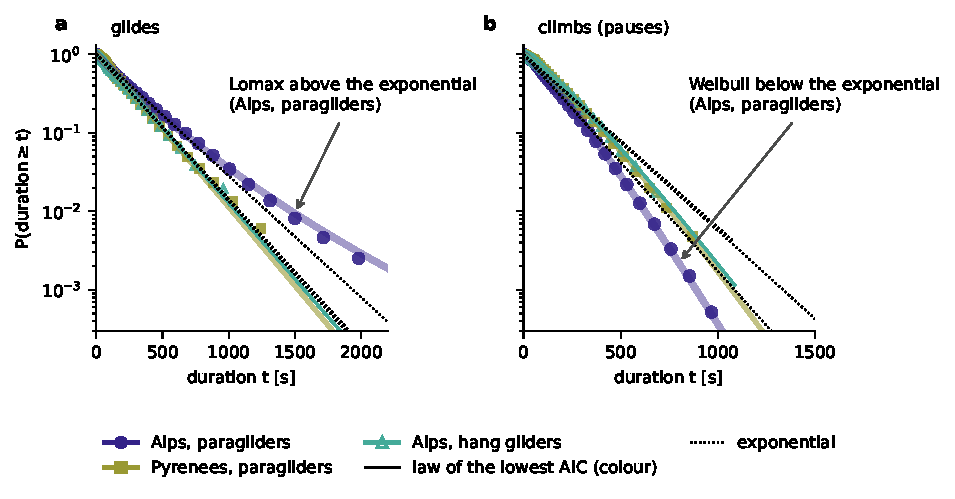
\includegraphics[width=\textwidth]{figures/flights_phases}
\caption{Glide and climb durations follow a law of lowest AIC close to the exponential, and the Weibull law fits the climbs. Survival $P(\text{duration} \ge t)$ on a logarithmic axis against a linear duration, where an exponential is a straight line, for the glides (a) and the climbs (b) of each group; markers: data (open for the hang gliders), coloured lines: the law of lowest AIC of Eq.~\eqref{eq:laws}, dotted black lines: exponential fit. Only the glides of the Alps paragliders leave the exponential upwards (Lomax tail); the climbs of all groups fall below it (Weibull, $k > 1$).}
\label{fig:flphases}
\end{figure}

\begin{table}[t]
\centering
\caption{Fits of Eq.~\eqref{eq:laws}: the law of lowest AIC with its parameters, and $\Delta\mathrm{AIC}$ of each of the four laws from the best (0 = best). Intervals: 95\%, bootstrap over flights.}
\label{tab:flfits}
\scriptsize
\setlength{\tabcolsep}{1.5pt}
\begin{tabular}{llrllrrrr}
\toprule
group & phase & mean (s) & law & parameters & Lomax & exp. & Weibull & gamma \\
\midrule
Alps, paragliders & glide & 281 & Lomax & $\mu$ = 10.11 (9.69--10.57); $\tau_0$ = 2555 (2437--2685) & 0 & 3417 & 1776 & 2635 \\
Alps, paragliders & pause & 158 & Weibull & $k$ = 1.150 (1.145--1.154); $\lambda$ = 165 (165--166) & 9134 & 9105 & 0 & 1796 \\
Alps, hang gliders & glide & 236 & gamma & $a$ = 1.057 (1.012--1.104); $\theta$ = 223 (211--233) & 9 & 7 & 2 & 0 \\
Alps, hang gliders & pause & 198 & Weibull & $k$ = 1.155 (1.125--1.188); $\lambda$ = 207 (199--214) & 160 & 157 & 0 & 49 \\
Pyrenees, paragliders & glide & 233 & gamma & $a$ = 1.089 (1.068--1.110); $\theta$ = 214 (208--220) & 103 & 106 & 47 & 0 \\
Pyrenees, paragliders & pause & 194 & Weibull & $k$ = 1.166 (1.152--1.180); $\lambda$ = 204 (201--207) & 937 & 933 & 0 & 202 \\
\bottomrule
\end{tabular}

\end{table}

The climbs of every group follow a Weibull law with $k$ above 1: $k = \flPauseParamAAlpsPara$ for the Alps paragliders (interval
\flPauseParamAAlpsParaLo{} to \flPauseParamAAlpsParaHi), \flPauseParamAAlpsHang{} for the Alps hang gliders and
\flPauseParamAPyrPara{} for the Pyrenees paragliders. A tail lighter than the exponential means that long climbs are rarer than
an exponential of the same mean predicts. The exponential is worse than the Weibull by \flPauseAicExpAlpsPara{} units of AIC for the
Alps paragliders and by \flPauseAicExpAlpsHang{} and \flPauseAicExpPyrPara{} for the other two groups, and the Lomax law, which
has a heavy tail, by more. The mean climb is \flPauseMeanAlpsPara~s, \flPauseMeanAlpsHang~s and \flPauseMeanPyrPara~s. The glides
of the Alps paragliders follow a Lomax law with $\mu = \flGlideParamAAlpsPara$ (\flGlideParamAAlpsParaLo{} to \flGlideParamAAlpsParaHi)
and $\tau_0 = \flGlideParamBAlpsPara$~s, whose tail is heavier than the exponential's ($\Delta\mathrm{AIC}$ of the exponential:
\flGlideAicExpAlpsPara); those of the Alps hang gliders and the Pyrenees paragliders follow a gamma law with $a$ close to
1 (\flGlideParamAAlpsHang{} and \flGlideParamAPyrPara), that is, nearly exponential, with mean glides of \flGlideMeanAlpsHang~s and
\flGlideMeanPyrPara~s. All fitted laws have a finite mean, so the progress along the route is ballistic again at lags much longer
than a glide and a climb.

\paragraph{What we keep.} The climbs are not exponential: their law is Weibull with $k \approx 1.15$ in every group, so that
long climbs are rarer than for an exponential. The glides are exponential or nearly so, except for the Alps paragliders, where
a Lomax tail wins by AIC. The model of Section~\ref{sec:flmodel} draws from the law of lowest AIC of each group and phase.

\subsection{An intermittent ball on the crests}\label{sec:flmodel}

What does the geometry give when the ball does not move at constant speed but stops as the pilot does? The ball
runs on a crest path $\mathbf p(s)$ of the region, with $s$ the arc length, and alternates glides and pauses. In
a glide it advances at the speed $v$ of Eq.~\eqref{eq:vglide}; in a pause it stays where it is. The searches of the flights are not in the model: the time a pilot spends
searching is dropped from its clock. The glide and
pause durations are independent draws of the laws of Eq.~\eqref{eq:laws} of lowest AIC, fitted on the glides and the climbs of the
flights of the same region and discipline, conditional on exceeding $X_0$:
\begin{equation}
  T = S^{-1}(U),\qquad U \text{ uniform on } (0,1),
  \label{eq:draw}
\end{equation}
rounded to whole seconds. The position at time $t$ is $\mathbf r(t) = \mathbf p\bigl(v\,\Theta(t)\bigr)$, where
$\Theta(t)$ is the time spent gliding up to $t$. The ball starts in equilibrium: the first phase is a glide with
probability $E[T_g]/(E[T_g] + E[T_p])$, and the time left in it has the density $S(t)/E[T]$ of the law of that
phase. The ball stops when it reaches the end of the path. Positions are given every second. Figure~\ref{fig:flmodels} draws the crest model beside the crests at constant speed and
the two null models of Section~\ref{sec:flnull}.

\begin{figure}[t]
\centering
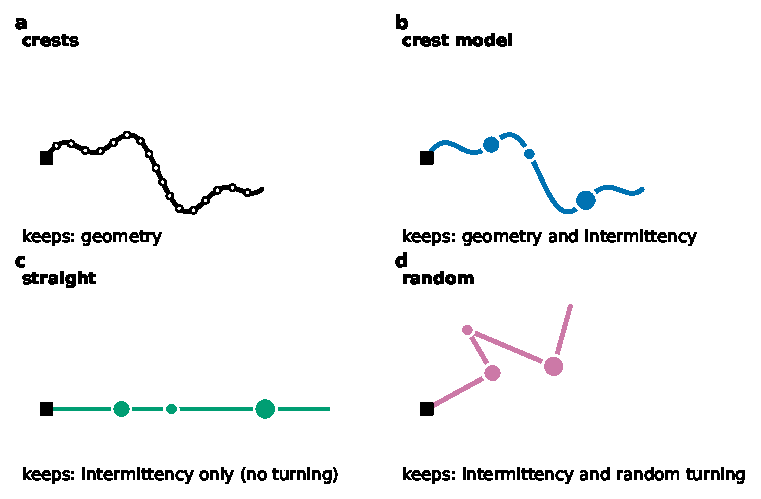
\includegraphics[width=\textwidth]{figures/flights_models}
\caption{The four motions differ only in what they keep of the flight. The same sequence of four glides and three pauses on
each model: the crests at constant speed (a, white dots at equal steps of time), the crest model (b), the straight model (c)
and the random model (d). Dot area: duration of the pause; black square: start.}
\label{fig:flmodels}
\end{figure}

The paths are all the joined paths of the region, those of Section~\ref{crest-sec:trees} of the crest report: \flNPathsAlpsPara{} in the
Alps and \flNPathsPyrPara{} in the Pyrenees, the same rows as the TAMSD of the crests, so that $\Hgeo$ and the
model have the same population. For each path we draw \flNReal{} realisations and pool their pairs. The TAMSD
$\delta^2_{\mathrm{mod}}(\tau)$ is Eq.~\eqref{crest-eq:tamsd} of the crest report at a lag of $\tau$ seconds, on 80 log-spaced lags up to a
quarter of the realisation, and the mean is taken with equal weight per path (Eq.~\eqref{crest-eq:mean} of the crest report). The
bootstrap draws whole trees, with the same draws for the crests and for the model, so that the difference
$\Hgeo - \Hmod$ is a paired one.

\paragraph{What we keep.} The model has two ingredients that come from the flights, the speed $v$ and the laws of
glides and pauses, and one from the ground, the path. On a straight line and with no pause it gives $\Hmod = 1$
(tests of \code{test\_model.py}).

\subsection{The curves of crests, model and flights}\label{sec:flcurves}

How do the mean squared displacements of the crests, the model and the flights compare, and where does each stop
being ballistic? Four curves are drawn for each region and discipline, all as functions of the lag $\tau$:
\begin{itemize}[nosep]
  \item \emph{crests}: $\overline{\delta^2}(s)$ of the crest paths, Eq.~\eqref{crest-eq:mean} of the crest report, at $\tau = s/v$;
  \item \emph{model}: $\overline{\delta^2_{\mathrm{mod}}}(\tau)$ of the intermittent ball;
  \item \emph{flights} (dyn): the TAMSD of the positions every second, circles included;
  \item \emph{flights} (route): the track in arc length with every thermalling circle replaced by its chord, at
        $\tau = s/v$ (Section~\ref{crest-sec:flcurves} of the crest report).
\end{itemize}
The two null models of Section~\ref{sec:flnull}, straight and random, are drawn in the same figures and fitted by the
same rule. Figure~\ref{fig:flmsd} plots the ratio $\overline{\delta^2}(\tau)/(v\tau)^2$, which is 1 for a ballistic motion at
speed $v$, and Figure~\ref{fig:flalpha} the local slope of the MSD
\begin{equation}
  \alpha(\tau) = \frac12\,\frac{d\ln\overline{\delta^2}}{d\ln\tau},
  \label{eq:alpha}
\end{equation}
which is Eq.~\eqref{crest-eq:alphaloc} of the crest report in time. The bands are the 2.5\% and 97.5\% percentiles of the bootstrap.

\paragraph{One rule for the exponent.} The rule is that of Section~\ref{crest-sec:flcurves} of the crest report. The fit of $H$ starts at the end of the initial ballistic regime. For each
curve, $H$ is half the least-squares slope of $\ln\overline{\delta^2}$ against $\ln\tau$ over the lags
$\tau_a \le \tau \le \tau_b$, where $\tau_a$ is the first lag not below $\flFloorM/v$ at which
$\alpha(\tau) < \flAlphaEnd$, and $\tau_b$ is the last lag that at least \flMinRows{} flights or paths reach, in every curve of the group
(\flTauMaxAlpsPara~s for the Alps paragliders). The floor of $\flFloorM$~m is the start of the fit of
Section~\ref{crest-sec:tamsd} of the crest report, converted to time. The rule is applied to the four curves alike and again in every
resample. For the Alps paragliders it starts the fit of the flights at \flStartDynAlpsPara~s, that of the model at \flStartModAlpsPara~s
and that of the crests at \flStartGeoAlpsPara~s: the floor decides, and the four curves are fitted over the same
range of lags within about a second. Table~\ref{tab:flh} gives $H$, and
Table~\ref{tab:flwindows} in Section~\ref{sec:flwindows} the fits on fixed windows of arc length.

\begin{figure}[t]
\centering
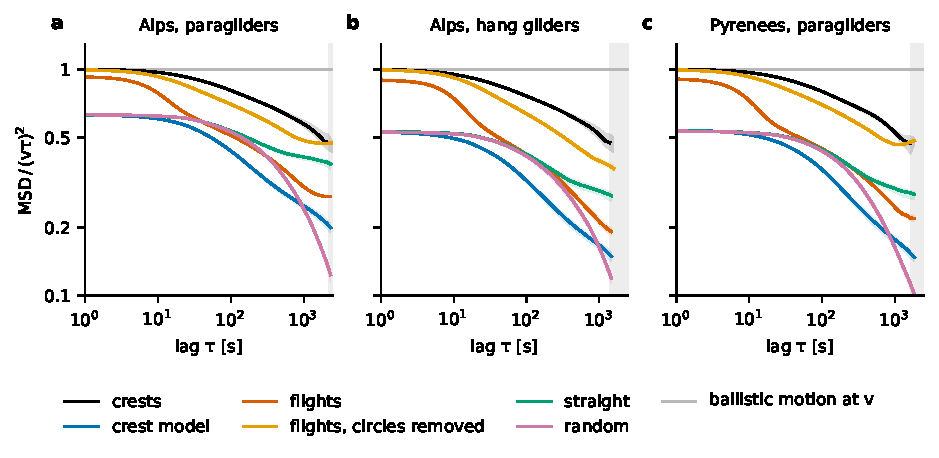
\includegraphics[width=\textwidth]{figures/flights_msd}
\caption{The crests stay closest to ballistic motion; pauses and turns lower the MSD of everything else. Mean squared displacement over the ballistic value, $\overline{\delta^2}(\tau)/(v\tau)^2$, of the crests, the crest model, the flights and the two null models against the lag $\tau$; grey line: 1, a ballistic motion at speed $v$. The crest model, the straight model and the random model start near 0.5 to 0.6 at a lag of 1~s because the ball is still during the pauses, so only the share of time spent gliding contributes. Bands: 95\% bootstrap intervals; grey zone: beyond the last lag of the fit.}
\label{fig:flmsd}
\end{figure}

\begin{figure}[t]
\centering
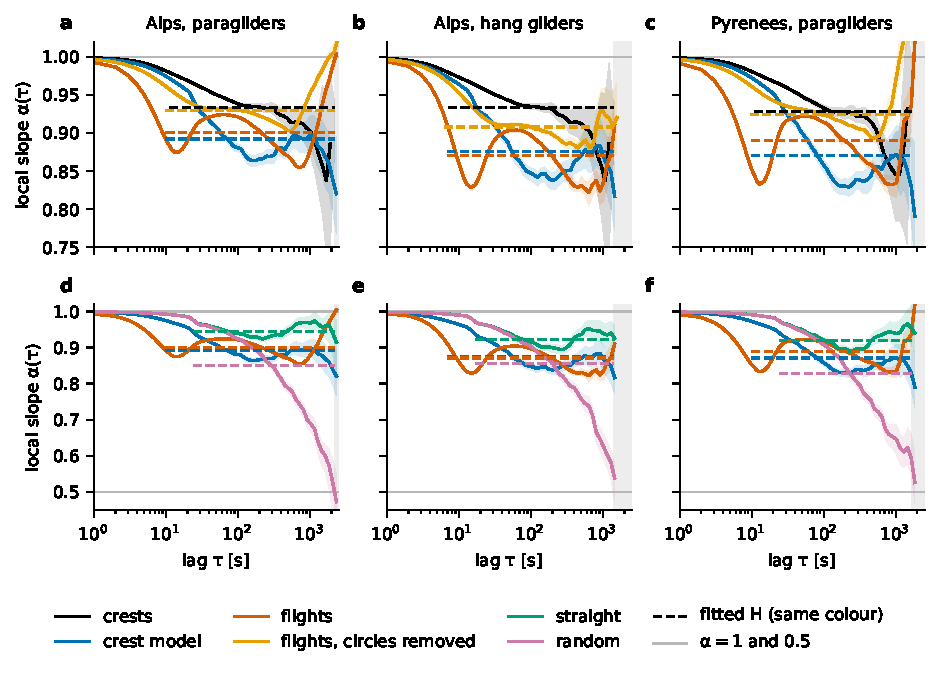
\includegraphics[width=\textwidth]{figures/flights_alpha}
\caption{The flights leave the ballistic regime within seconds; the crest model, the straight model and the random model bracket
them. Local slope of the MSD, $\alpha(\tau)$, Eq.~\eqref{eq:alpha}, against the lag $\tau$, for the Alps paragliders (a, d), the Alps
hang gliders (b, e) and the Pyrenees paragliders (c, f). Top row: crests, crest model, flights and flights without circles. Bottom
row: the straight and random null models against the flights and the crest model. Thin grey lines: $\alpha = 1$ (ballistic) and,
for the null models, $0.5$ (diffusive). Dashed horizontal lines: $H$ of the fit of the rule of the text (Table~\ref{tab:flh}), in the
colour of the curve, over the lags of the fit; for the Alps paragliders the crests give \flHGeoAlpsPara, the crest model
\flHModAlpsPara, the flights \flHDynAlpsPara, the flights without circles \flHRouteAlpsPara, the straight model \flHStraightAlpsPara{}
and the random model \flHRandomAlpsPara. Curves stop where fewer than \flMinRows{} flights or paths reach the lag, and the grey zone
is beyond the last lag of the fit. The Alps hang gliders rest on \flNAlpsHang{} flights and are noisier. Bands: 95\% bootstrap
intervals.}
\label{fig:flalpha}
\end{figure}

\begin{table}[t]
\centering
\caption{$H$ of the curves, fitted by the rule of the text, with 95\% intervals: crests, crest model, flights (dyn), route
of the flights and the two null models. The flights are all those of the group that pass the selection (not only those
at 1~Hz).}
\label{tab:flh}
\scriptsize
\setlength{\tabcolsep}{2pt}
\begin{tabular}{llll}
\toprule
curve & Alps, paragliders & Alps, hang gliders & Pyrenees, paragliders \\
\midrule
number of flights & 23320 & 784 & 2140 \\
crests & 0.934 (0.930--0.940) & 0.934 (0.930--0.940) & 0.929 (0.926--0.933) \\
crest model & 0.892 (0.888--0.896) & 0.876 (0.871--0.880) & 0.871 (0.866--0.874) \\
flights & 0.901 (0.901--0.902) & 0.871 (0.869--0.874) & 0.890 (0.888--0.892) \\
flights, circles removed & 0.929 (0.929--0.930) & 0.908 (0.906--0.910) & 0.925 (0.923--0.926) \\
straight & 0.945 (0.941--0.947) & 0.923 (0.918--0.927) & 0.921 (0.915--0.924) \\
random & 0.849 (0.844--0.852) & 0.857 (0.853--0.862) & 0.829 (0.823--0.833) \\
\bottomrule
\end{tabular}

\end{table}

For the Alps paragliders the crests give $\Hgeo = \flHGeoAlpsPara$, the model $\Hmod = \flHModAlpsPara$, the
flights $\Hdyn = \flHDynAlpsPara$ and the route of the flights $\Hroute = \flHRouteAlpsPara$. The route of the
Pyrenees paragliders, $\flHRoutePyrPara$, is close to its crests, $\flHGeoPyrPara$; that of the Alps hang gliders,
$\flHRouteAlpsHang$, is lower than its crests, $\flHGeoAlpsHang$. The curves of $\alpha$ show where $\Hdyn$ and
$\Hroute$ differ: the flights leave the ballistic value at about the floor, fall to a minimum within the first
twenty seconds, which is about half a turn of a circle, and then recover part of the way; the route has no such
minimum. The model has no circles and its $\alpha$ falls steadily with the lag; after the circles it is below the
flights at the shorter lags and comes close to them at the longer ones. Towards $\tau_b$ the curves of the flights rise, because only the longest flights reach these lags and these are the
straightest; the fit stops at $\tau_b$.

\paragraph{What we keep.} The crests, the route of the flights, the flights with their circles and the model are
four different curves. The route of the paragliders follows the crests as straight as the crests are, and the
route of the hang gliders is a little less straight. The circles lower $H$ from the route
($\Hroute = \flHRouteAlpsPara$ for the Alps paragliders) to the flights ($\Hdyn = \flHDynAlpsPara$). The model's $H$ is below that of the flights for the paragliders of both massifs ($\Hmod = \flHModAlpsPara$ against
$\Hdyn = \flHDynAlpsPara$ in the Alps and \flHModPyrPara{} against \flHDynPyrPara{} in the Pyrenees) and above it
for the Alps hang gliders (\flHModAlpsHang{} against \flHDynAlpsHang{}).

\subsection{Splitting \texorpdfstring{$1-H$}{1 - H}}\label{sec:fldecomp}

How much of $1-\Hdyn$ is geometry, how much intermittency, and how much is left? With $\Hdyn$ the exponent of the
flights, the identity
\begin{equation}
  1 - \Hdyn = (1 - \Hgeo) + (\Hgeo - \Hmod) + (\Hmod - \Hdyn)
  \label{eq:split}
\end{equation}
splits the deficit into the part of the crests, the part that the model adds by stopping, and what remains. Each
term is given as a percentage of $1 - \Hdyn$. The intervals come from the joint bootstrap: the same draw of trees
for $\Hgeo$ and $\Hmod$, and a draw of flights for $\Hdyn$. Figure~\ref{fig:fldecomp} and
Table~\ref{tab:fldecomp} give the result.

\begin{figure}[t]
\centering
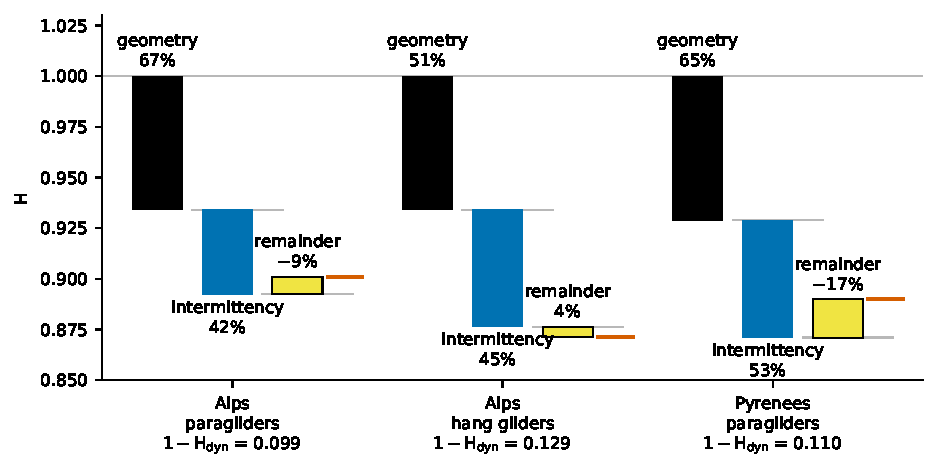
\includegraphics[width=\textwidth]{figures/flights_decomposition}
\caption{Geometry and intermittency each take a large part of $1 - \Hdyn$, and the remainder is small. From $H = 1$ down to
$\Hdyn$ in three steps, $1 - \Hgeo$, $\Hgeo - \Hmod$ and $\Hmod - \Hdyn$ (Eq.~\eqref{eq:split}); each step is labelled with its
share of $1 - \Hdyn$. The last step goes up when $\Hmod < \Hdyn$, and its share is then negative. Intervals are in
Table~\ref{tab:fldecomp}.}
\label{fig:fldecomp}
\end{figure}

\begin{table}[t]
\centering
\caption{Terms of Eq.~\eqref{eq:split}. A negative remainder means $\Hmod < \Hdyn$: the model has less exponent
than the flights. The Pyrenees hang gliders have \flSelPyrHang{} flights that pass the selection and
\flNOneHzPyrHang{} with phases at 1~Hz, and are not analysed.}
\label{tab:fldecomp}
\small
\begin{tabular}{lrrlll}
\toprule
group & flights & $1-\Hdyn$ & geometry (\%) & intermittency (\%) & remainder (\%) \\
\midrule
Alps, paragliders & 23320 & 0.099 & 67 (60--71) & 42 (39--49) & $-$9 ($-$13 to $-$6) \\
Alps, hang gliders & 784 & 0.129 & 51 (46--55) & 45 (41--51) & 4 (0 to 7) \\
Pyrenees, paragliders & 2140 & 0.110 & 65 (60--68) & 53 (48--59) & $-$17 ($-$22 to $-$14) \\
\bottomrule
\end{tabular}

\end{table}

For the Alps paragliders $1 - \Hdyn = \flTotalAlpsPara$, of which the crests carry \flPctGeometryAlpsPara\%
(interval \flPctGeometryAlpsParaLo\% to \flPctGeometryAlpsParaHi\%), the stops of the model
\flPctInterAlpsPara\% (\flPctInterAlpsParaLo\% to \flPctInterAlpsParaHi\%) and the remainder is
\flPctOtherAlpsPara\% (\flPctOtherAlpsParaLo\% to \flPctOtherAlpsParaHi\%). The Pyrenees paragliders give
\flPctGeometryPyrPara\%, \flPctInterPyrPara\% and \flPctOtherPyrPara\%. The Alps hang gliders give
\flPctGeometryAlpsHang\%, \flPctInterAlpsHang\% and \flPctOtherAlpsHang\% (interval \flPctOtherAlpsHangLo\% to
\flPctOtherAlpsHangHi\%, which reaches zero).

For the paragliders the remainder is negative and the first two terms add to more than 100\%: the model falls
below the flights, so a ball that stops completely for the observed climbs loses more exponent than the flights
lose. We have not tested why. A possible reason is that a pilot in a climb is not at rest, since he circles and
drifts with the thermal, but the model does not move at all in a pause. For these groups the shares are the
shares of a model that overshoots, and the remainder is the size of the overshoot. For the Alps hang gliders the
remainder is positive but its interval reaches zero, so the model and the flights agree within the interval. Fitting the climbs
by Weibull laws that follow their whole survival, in place of the exponential and Lomax laws used first, left the remainder
unchanged to within one percentage point in every group: the tail of the climb law does not explain the overshoot.
The Alps hang gliders have a smaller geometric share than the paragliders, because their $1 - \Hdyn$ is larger.

A first version of the model used search and climb runs joined as the pause. It gave $\Hmod = \flHModOldAlpsPara$,
$\flHModOldPyrPara$ and $\flHModOldAlpsHang$ for the Alps paragliders, the Pyrenees paragliders and the Alps hang
gliders, intermittency shares of \flPctInterOldAlpsPara\%, \flPctInterOldPyrPara\% and \flPctInterOldAlpsHang\%
and remainders of \flPctOtherOldAlpsPara\%, \flPctOtherOldPyrPara\% and \flPctOtherOldAlpsHang\%: a longer
pause lowered the model further below the flights.

The two null models of Section~\ref{sec:flnull} stand \flNullGapStraightAlpsPara\% (straight) and
\flNullGapRandomAlpsPara\% (random) of $1-\Hdyn$ from the flights for the Alps paragliders, \flNullGapStraightAlpsHang\% and
\flNullGapRandomAlpsHang\% for the Alps hang gliders and \flNullGapStraightPyrPara\% and \flNullGapRandomPyrPara\% for the
Pyrenees paragliders.

\paragraph{What we keep.} The crests carry \flPctGeometryAlpsPara\%, \flPctGeometryPyrPara\% and
\flPctGeometryAlpsHang\% of $1 - \Hdyn$ for the Alps paragliders, the Pyrenees paragliders and the Alps hang
gliders. The stops of the model take \flPctInterAlpsPara\%, \flPctInterPyrPara\% and \flPctInterAlpsHang\%, and
the remainder is \flPctOtherAlpsPara\%, \flPctOtherPyrPara\% and \flPctOtherAlpsHang\%. The model falls below
the flights for the paragliders and agrees with them, within the interval, for the Alps hang gliders. The split
is a statement about this model, and the Pyrenees hang gliders are too few to say anything.

\subsection{Two null models without the crest geometry}\label{sec:flnull}

Is the crest geometry needed, or do the pauses and the glide lengths alone give the exponent of the flights? Two null
models keep everything of the crest model except the geometry of the motion: the glide and climb laws of
Eq.~\eqref{eq:laws} of the group, the speed $v$, the still pauses, the \flNReal{} realisations per path, the length of
the path (the ball stops when it has glided that distance), the TAMSD and the rule of the fit. In the \emph{straight}
model every glide goes on along one fixed line, so that $\mathbf r(t) = (v\,\Theta(t),\,0)$ with $\Theta(t)$ the time
spent gliding. In the \emph{random} model glide $i$ is a straight segment in a direction $\theta_i$ drawn uniformly on the
circle, independent of the previous one: $\mathbf r(t) = v\sum_i \Theta_i(t)\,(\cos\theta_i, \sin\theta_i)$, where
$\Theta_i(t)$ is the time spent in glide $i$ up to $t$. The straight model is the extreme of a ball that never turns and
the random model that of a ball that forgets its direction at every glide. Figures~\ref{fig:flmsd} and~\ref{fig:flalpha}
show them with the other curves and Table~\ref{tab:flh} their $H$. Table~\ref{tab:flnulls} gives how far each is from the
flights, as $\Delta H = H_{\mathrm{null}} - \Hdyn$ and as the gap $100\,\Delta H/(1-\Hdyn)$ in percent.

\begin{table}[t]
\centering
\caption{$H$ of the null models and their distance to the flights: $\Delta H$ and the gap as a percentage of
$1-\Hdyn$, with 95\% intervals. A positive gap means $H$ above the flights.}
\label{tab:flnulls}
\scriptsize
\setlength{\tabcolsep}{2pt}
\begin{tabular}{llll}
\toprule
null model & Alps, paragliders & Alps, hang gliders & Pyrenees, paragliders \\
\midrule
straight: $H$ & 0.945 (0.941--0.947) & 0.923 (0.918--0.927) & 0.921 (0.915--0.924) \\
straight: $\Delta H$ & 0.044 (0.040--0.046) & 0.052 (0.047--0.056) & 0.031 (0.025--0.035) \\
straight: gap (\%) & 44 (40--47) & 40 (36--43) & 28 (23--31) \\
random: $H$ & 0.849 (0.844--0.852) & 0.857 (0.853--0.862) & 0.829 (0.823--0.833) \\
random: $\Delta H$ & $-$0.052 ($-$0.057 to $-$0.049) & $-$0.014 ($-$0.019 to $-$0.009) & $-$0.061 ($-$0.067 to $-$0.056) \\
random: gap (\%) & $-$53 ($-$57 to $-$50) & $-$11 ($-$15 to $-$7) & $-$55 ($-$61 to $-$51) \\
\bottomrule
\end{tabular}

\end{table}

For the Alps paragliders the straight model has $H = \flHStraightAlpsPara$, above the crests ($\Hgeo = \flHGeoAlpsPara$),
above the crest model ($\flHModAlpsPara$) and above the flights ($\Hdyn = \flHDynAlpsPara$), by $\Delta H =
\flNullDHStraightAlpsPara$. The random model has $H = \flHRandomAlpsPara$, below the flights by $\flNullDHRandomAlpsPara$
(a gap of \flNullGapRandomAlpsPara\%). The crest model lies between the two, and so do the flights, in all three groups. The
straight model shows that the pauses alone lower $H$ to this value, since a ball that never turns has $\alpha = 1$ without
them, and its $\alpha$ tends to 1 at lags much longer than a glide and a climb. Where fewer than \flMinRows{} paths reach a lag, the
curves of the crest model and of the straight model drop, because only the paths with the most pauses are long enough to reach
it; the figures stop before this. In the random model $\alpha$ keeps falling with the lag, towards 0.5 for lags much longer than a glide
(Figure~\ref{fig:flalpha}), where the flights and the crest model do not. For the hang gliders the random model comes
closer to the flights (gap \flNullGapRandomAlpsHang\%) than for the paragliders, but still below them, and its $\alpha$ has the
same continuing fall.

\paragraph{What we keep.} The two extremes bracket the flights: a ball that never turns has $H$ above them, a ball that
forgets its direction at every glide has $H$ below them, and the crest model lies in between. The crest geometry
therefore matters: the same durations and speed give $H$ from \flHRandomAlpsPara{} to \flHStraightAlpsPara{} for the Alps
paragliders according to the geometry of the motion, and the crests put it at \flHModAlpsPara, close to the flights' \flHDynAlpsPara.

\subsection{Fixed windows of arc length}\label{sec:flwindows}

Does the picture of the rule change on fixed windows? Table~\ref{tab:flwindows} gives $H$ of the four curves on
the windows of Table~\ref{crest-tab:hgeo} of the crest report, divided by $v$ to give lags. The window from 0.1~km starts at the floor and each curve runs to its last lag with
at least \flMinRows{} flights or paths, not to $\tau_b$.

\begin{table}[t]
\centering
\caption{$H$ on fixed windows of arc length $s = v\tau$, with 95\% intervals.}
\label{tab:flwindows}
\scriptsize
\setlength{\tabcolsep}{2pt}
\begin{tabular}{llllll}
\toprule
group & window of $s$ (km) & $\Hgeo$ & $\Hmod$ & $\Hdyn$ & $\Hroute$ \\
\midrule
Alps, paragliders & 0.1-inf & 0.935 (0.930--0.941) & 0.888 (0.884--0.892) & 0.921 (0.920--0.922) & 0.944 (0.941--0.945) \\
Alps, paragliders & 0.1-1 & 0.961 (0.960--0.962) & 0.929 (0.926--0.931) & 0.909 (0.908--0.909) & 0.938 (0.937--0.938) \\
Alps, paragliders & 1-10 & 0.927 (0.921--0.934) & 0.876 (0.870--0.882) & 0.885 (0.885--0.886) & 0.916 (0.915--0.917) \\
Alps, paragliders & 10-inf & 0.870 (0.814--0.938) & 0.844 (0.809--0.893) & 1.060 (1.050--1.071) & 1.042 (1.025--1.048) \\
Alps, hang gliders & 0.1-inf & 0.935 (0.930--0.941) & 0.869 (0.864--0.874) & 0.871 (0.868--0.875) & 0.908 (0.905--0.911) \\
Alps, hang gliders & 0.1-1 & 0.961 (0.960--0.962) & 0.929 (0.926--0.932) & 0.865 (0.862--0.868) & 0.929 (0.927--0.931) \\
Alps, hang gliders & 1-10 & 0.927 (0.921--0.934) & 0.848 (0.840--0.854) & 0.867 (0.865--0.870) & 0.897 (0.894--0.900) \\
Alps, hang gliders & 10-inf & 0.870 (0.815--0.935) & 0.822 (0.786--0.872) & 0.903 (0.880--0.928) & 0.926 (0.904--0.948) \\
Pyrenees, paragliders & 0.1-inf & 0.930 (0.927--0.935) & 0.865 (0.860--0.868) & 0.900 (0.897--0.903) & 0.933 (0.930--0.935) \\
Pyrenees, paragliders & 0.1-1 & 0.960 (0.958--0.961) & 0.928 (0.924--0.931) & 0.897 (0.896--0.899) & 0.938 (0.937--0.939) \\
Pyrenees, paragliders & 1-10 & 0.917 (0.912--0.923) & 0.841 (0.832--0.847) & 0.873 (0.871--0.875) & 0.908 (0.905--0.910) \\
Pyrenees, paragliders & 10-inf & 0.886 (0.778--0.961) & 0.814 (0.750--0.880) & 1.036 (1.013--1.061) & 1.045 (1.024--1.064) \\
\bottomrule
\end{tabular}

\end{table}

The window beyond 10~km gives $H$ above 1 for the flights and the route of the paragliders. We attribute it to
the selection of the longest flights at these lags, since only they reach them, and we do not interpret it. On the window from 0.1 to 1~km the model is above the flights, as expected for a ball without
circles; on the window from 1 to 10~km it is below the flights, and the route is above both.

\paragraph{What we keep.} On the window from 1 to 10~km the order is the same as for the rule: the model below
the flights and the flights below the route. On the window from 0.1 to 1~km the model is above the flights, which
is consistent with the circles of the flights bending them at these scales while the model has none. The window
beyond 10~km is not interpreted.


\end{document}
